% =====================================================================
% ELMED219: Nevrale nettverk og dyplæring
% Beamer-presentasjon - Momentliste D01-D13
% =====================================================================
\documentclass[aspectratio=169, 10pt]{beamer}

% =====================================================================
% PAKKER
% =====================================================================
\usepackage[utf8]{inputenc}
\usepackage[T1]{fontenc}
\usepackage[norsk]{babel}
\usepackage{graphicx}
\usepackage{tikz}
\usetikzlibrary{shapes.geometric, arrows, positioning, calc, decorations.pathreplacing}
\usepackage{booktabs}
\usepackage{amsmath}
\usepackage{fontawesome5}

% =====================================================================
% TEMA OG FARGER
% =====================================================================
\usetheme{Madrid}
\usecolortheme{beaver}

% Farger for TikZ-diagrammer
\definecolor{uibblue}{RGB}{0, 61, 115}
\definecolor{uibred}{RGB}{175, 28, 44}

% =====================================================================
% TITTELINFO
% =====================================================================
\title{Nevrale nettverk og Dyplæring}
\subtitle{ELMED219: Momentliste D01--D13}
\author{ELMED219}
\date{Vår 2026}

% =====================================================================
% DOKUMENT
% =====================================================================
\begin{document}

% Tittelside
\begin{frame}
    \titlepage
\end{frame}

% Innholdsfortegnelse
\begin{frame}{Oversikt}
    \tableofcontents
\end{frame}

% =====================================================================
% SEKSJON: Biologiske vs. kunstige nevroner
% =====================================================================
\section{Grunnleggende nevrale nettverk}

\begin{frame}{D01: Sammenligne biologiske og kunstige nevroner}
    \begin{columns}[T]
        \begin{column}{0.48\textwidth}
            \textbf{Biologisk nevron:}
            \begin{itemize}
                \item \textbf{Dendritter:} Mottar signaler
                \item \textbf{Cellekropp:} Prosesserer
                \item \textbf{Akson:} Sender videre
                \item \textbf{Synapse:} Kobling til neste nevron
                \item Kompleks elektrokjemisk aktivitet
            \end{itemize}
        \end{column}
        \begin{column}{0.48\textwidth}
            \textbf{Kunstig nevron (perseptron):}
            \begin{itemize}
                \item \textbf{Inputs} $x_1, x_2, \ldots$: Mottar data
                \item \textbf{Vekter} $w_1, w_2, \ldots$: Synapsestyrke
                \item \textbf{Sum:} $z = \sum w_i x_i + b$
                \item \textbf{Aktivering:} $a = f(z)$ \small(f = aktiveringsfunksjon)
                \item Matematisk forenkling
            \end{itemize}
        \end{column}
    \end{columns}
    
    \vspace{0.5cm}
    \begin{block}{Nøkkellikhet}
        Begge summerer inngående signaler og ``fyrer'' (aktiverer) hvis total stimulering overstiger en terskel.
    \end{block}
    
    \begin{alertblock}{Viktig forskjell}
        Kunstige nevroner er \textbf{kraftig forenklede modeller} -- de fanger ikke hjernens fulle kompleksitet.
    \end{alertblock}
\end{frame}

\begin{frame}{D02: Beskrive oppbygningen av et multilags perseptron (MLP)}
    \begin{columns}[T]
        \begin{column}{0.55\textwidth}
            \textbf{MLP-arkitektur:}
            \begin{itemize}
                \item \textbf{Inputlag:} Mottar features (ikke prosessering)
                \item \textbf{Skjulte lag:} 1 eller flere lag med nevroner
                \item \textbf{Outputlag:} Produserer prediksjon
            \end{itemize}
            
            \vspace{0.3cm}
            \textbf{Fully connected (dense):}
            \begin{itemize}
                \item Hvert nevron i ett lag er koblet til \textbf{alle} nevroner i neste lag
                \item Mange parametre (vekter og bias)
            \end{itemize}
            
            \vspace{0.3cm}
            \textbf{``Dyp'' læring:}
            \begin{itemize}
                \item $\geq$ 2 skjulte lag = dyp modell
                \item Flere lag $\rightarrow$ mer abstrakte representasjoner
            \end{itemize}
        \end{column}
        \begin{column}{0.42\textwidth}
            \begin{tikzpicture}[scale=0.7, transform shape]
                \tikzstyle{neuron}=[circle, draw=uibblue, fill=uibblue!20, minimum size=0.6cm]
                
                % Input layer
                \foreach \y in {1,2,3} {
                    \node[neuron] (i\y) at (0, -\y) {};
                }
                \node at (0, -4.2) {\footnotesize Input};
                
                % Hidden layer 1
                \foreach \y in {0.5,1.5,2.5,3.5} {
                    \node[neuron, fill=uibblue!40] (h1\y) at (2, -\y) {};
                }
                \node at (2, -4.7) {\footnotesize Skjult 1};
                
                % Hidden layer 2
                \foreach \y in {1,2,3} {
                    \node[neuron, fill=uibblue!60] (h2\y) at (4, -\y) {};
                }
                \node at (4, -4.2) {\footnotesize Skjult 2};
                
                % Output layer
                \foreach \y in {1.5,2.5} {
                    \node[neuron, fill=uibred!40] (o\y) at (6, -\y) {};
                }
                \node at (6, -4.2) {\footnotesize Output};
                
                % Connections (simplified)
                \foreach \i in {1,2,3} {
                    \foreach \h in {0.5,1.5,2.5,3.5} {
                        \draw[gray!50, thin] (i\i) -- (h1\h);
                    }
                }
                \foreach \ha in {0.5,1.5,2.5,3.5} {
                    \foreach \hb in {1,2,3} {
                        \draw[gray!50, thin] (h1\ha) -- (h2\hb);
                    }
                }
                \foreach \h in {1,2,3} {
                    \foreach \o in {1.5,2.5} {
                        \draw[gray!50, thin] (h2\h) -- (o\o);
                    }
                }
            \end{tikzpicture}
        \end{column}
    \end{columns}
\end{frame}

\begin{frame}{D03: Forklare hva en aktiveringsfunksjon er (ReLU, sigmoid)}
    \textbf{Hvorfor aktiveringsfunksjoner?} Uten dem: Hele nettverket = lineær transformasjon. Introduserer \textbf{ikke-linearitet}.

    \vspace{0.2cm}
    \begin{columns}[T]
        \begin{column}{0.48\textwidth}
            \textbf{Sigmoid:} $\sigma(z) = \frac{1}{1 + e^{-z}}$
            \begin{itemize}
                \item Output: $(0, 1)$
                \item Problem: \textit{vanishing gradients}
                \item Brukes i output for binær klassifisering
            \end{itemize}
        \end{column}
        \begin{column}{0.48\textwidth}
            \textbf{ReLU:} $\text{ReLU}(z) = \max(0, z)$
            \begin{itemize}
                \item Output: $[0, \infty)$
                \item Moderne standard for skjulte lag
                \item Rask, unngår vanishing gradients
            \end{itemize}
        \end{column}
    \end{columns}

    \vspace{0.2cm}
    \begin{block}{\footnotesize Softmax (multi-klasse output)}
        \footnotesize $\text{softmax}(z_i) = \frac{e^{z_i}}{\sum_j e^{z_j}}$ -- gir sannsynlighetsfordeling over klasser (summerer til 1)
    \end{block}
\end{frame}

% =====================================================================
% SEKSJON: Trening av nevrale nettverk
% =====================================================================
\section{Trening av nevrale nettverk}

\begin{frame}{D04: Forstå konseptet forward propagation}
    \textbf{Forward propagation = fremoverberegning}
    
    \begin{enumerate}
        \item \textbf{Input:} Data $\mathbf{x}$ (features) legges inn i inputlaget
        \item \textbf{For hvert lag:}
        \begin{itemize}
            \item Beregn vektet sum: $z^{(l)} = W^{(l)} \cdot a^{(l-1)} + b^{(l)}$
            \item Appliser aktivering: $a^{(l)} = f(z^{(l)})$
        \end{itemize}
        \item \textbf{Output:} Prediksjon $\hat{y}$ fra siste lag
    \end{enumerate}
    
    \vspace{0.3cm}
    \begin{center}
        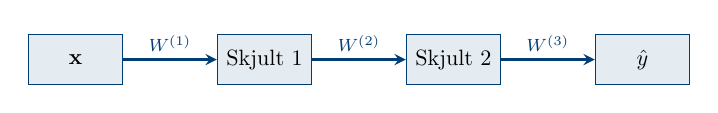
\begin{tikzpicture}[scale=0.8, transform shape]
            \tikzstyle{block} = [rectangle, draw=uibblue, fill=uibblue!10, minimum width=1.5cm, minimum height=0.8cm]
            \tikzstyle{arrow} = [thick,->,>=stealth,uibblue]
            
            \node[block] (x) at (0,0) {$\mathbf{x}$};
            \node[block] (h1) at (3,0) {Skjult 1};
            \node[block] (h2) at (6,0) {Skjult 2};
            \node[block] (y) at (9,0) {$\hat{y}$};
            
            \draw[arrow] (x) -- node[above] {\footnotesize $W^{(1)}$} (h1);
            \draw[arrow] (h1) -- node[above] {\footnotesize $W^{(2)}$} (h2);
            \draw[arrow] (h2) -- node[above] {\footnotesize $W^{(3)}$} (y);
        \end{tikzpicture}
    \end{center}
    
    \vspace{0.3cm}
    \begin{block}{Nøkkelpunkt}
        Forward propagation beregner prediksjon -- ingen læring skjer her. Læring skjer ved backpropagation og oppdatering av vekter.
    \end{block}
\end{frame}

\begin{frame}{D05: Forklare backpropagation på et konseptuelt nivå}
    \textbf{Backpropagation = bakoverberegning av feil}
    
    \vspace{0.3cm}
    \textbf{Hovedidé:}
    \begin{enumerate}
        \item \textbf{Beregn feil:} Sammenlign prediksjon $\hat{y}$ med fasit $y$
        \item \textbf{Propager bakover:} Hvor mye bidro hver vekt til feilen?
        \item \textbf{Kjerneregelen:} Deriver feil m.h.p. hver vekt i nettverket
        \item \textbf{Oppdater vekter:} Juster for å redusere feil
    \end{enumerate}
    
    \vspace{0.3cm}
    \begin{alertblock}{Intuisjon}
        Tenk deg at du justerer en kompleks maskin: Backpropagation forteller deg hvilke skruer (vekter) du skal skru på, og i hvilken retning, for å forbedre resultatet.
    \end{alertblock}
    
    \vspace{0.3cm}
    \begin{block}{Matematisk (forenklet)}
        $\frac{\partial L}{\partial w} = \frac{\partial L}{\partial \hat{y}} \cdot \frac{\partial \hat{y}}{\partial z} \cdot \frac{\partial z}{\partial w}$
        
        \small (Kjerneregelen for derivasjon propagerer gradienter bakover gjennom nettverket)
    \end{block}
\end{frame}

\begin{frame}{D06: Forstå gradient descent og læringsrate}
    \textbf{Gradient descent:}
    \begin{itemize}
        \item Optimiseringsalgoritme for å \textbf{minimere loss-funksjonen}
        \item Følger den \textbf{negative gradienten} (bratteste nedoverbakke)
    \end{itemize}
    
    \vspace{0.3cm}
    \textbf{Oppdateringsregel:}
    \[
    w_{\text{ny}} = w_{\text{gammel}} - \eta \cdot \frac{\partial L}{\partial w}
    \]
    
    \begin{columns}[T]
        \begin{column}{0.48\textwidth}
            \textbf{Læringsrate $\eta$:}
            \begin{itemize}
                \item Bestemmer \textbf{steglengde}
                \item For stor: Hopper over minimum
                \item For liten: Treg konvergens
                \item Typisk: 0.001--0.01
            \end{itemize}
        \end{column}
        \begin{column}{0.48\textwidth}
            \textbf{Varianter:}
            \begin{itemize}
                \item \textbf{Batch GD:} Alle data per oppdatering
                \item \textbf{Stochastic GD:} Ett eksempel om gangen
                \item \textbf{Mini-batch GD:} Små grupper (32--128)
                \item \textbf{Adam:} Adaptiv læringsrate (populær!)
            \end{itemize}
        \end{column}
    \end{columns}
    
    \vspace{0.2cm}
    \begin{block}{\footnotesize Epoch}
        \footnotesize En \textbf{epoch} = én gjennomgang av hele treningsdatasettet
    \end{block}
\end{frame}

\begin{frame}{D07: Kjenne til loss functions (cross-entropy, MSE)}
    \textbf{Loss function (tapsfunksjon):}
    \begin{itemize}
        \item Måler \textbf{hvor feil} modellens prediksjoner er
        \item Målet: Minimere loss under trening
    \end{itemize}
    
    \vspace{0.3cm}
    \begin{columns}[T]
        \begin{column}{0.48\textwidth}
            \textbf{MSE (Mean Squared Error):}
            \[
            L = \frac{1}{n}\sum_{i=1}^{n}(y_i - \hat{y}_i)^2
            \]
            \begin{itemize}
                \item Brukes for \textbf{regresjon}
                \item Straffes hardt for store feil
                \item Kontinuerlig output
            \end{itemize}
        \end{column}
        \begin{column}{0.48\textwidth}
            \textbf{Cross-Entropy:}
            \[
            L = -\sum_{i} y_i \log(\hat{y}_i)
            \]
            \begin{itemize}
                \item Brukes for \textbf{klassifisering}
                \item Binary: $-[y\log\hat{y} + (1-y)\log(1-\hat{y})]$
                \item Måler avvik mellom sannsynlighetsfordelinger
            \end{itemize}
        \end{column}
    \end{columns}
    
    \vspace{0.2cm}
    \begin{block}{\footnotesize Velge riktig loss}
        \footnotesize
        \textbf{Regresjon:} MSE/MAE \quad \textbf{Binær:} Binary CE \quad \textbf{Multi-klasse:} Categorical CE
    \end{block}
\end{frame}

% =====================================================================
% SEKSJON: Konvolusjonelle nevrale nettverk
% =====================================================================
\section{Konvolusjonelle nevrale nettverk (CNN)}

\begin{frame}{D08: Beskrive et konvolusjonelt nevralt nettverk (CNN)}
    \textbf{CNN = spesialisert for bildedata}
    
    \begin{itemize}
        \item Utnytter \textbf{romlig struktur} i bilder
        \item Langt færre parametre enn fullt koblet nettverk
        \item Translasjonsinvariant -- gjenkjenner mønstre uansett posisjon
    \end{itemize}
    
    \vspace{0.3cm}
    \textbf{Typisk CNN-arkitektur:}
    \begin{center}
        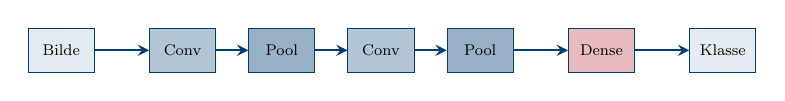
\begin{tikzpicture}[scale=0.7, transform shape]
            \tikzstyle{block} = [rectangle, draw=uibblue, fill=uibblue!10, minimum width=1.2cm, minimum height=0.8cm, font=\footnotesize]
            \tikzstyle{arrow} = [thick,->,>=stealth,uibblue]
            
            \node[block] (img) at (0,0) {Bilde};
            \node[block, fill=uibblue!30] (c1) at (2.2,0) {Conv};
            \node[block, fill=uibblue!40] (p1) at (4,0) {Pool};
            \node[block, fill=uibblue!30] (c2) at (5.8,0) {Conv};
            \node[block, fill=uibblue!40] (p2) at (7.6,0) {Pool};
            \node[block, fill=uibred!30] (fc) at (9.8,0) {Dense};
            \node[block] (out) at (12,0) {Klasse};
            
            \draw[arrow] (img) -- (c1);
            \draw[arrow] (c1) -- (p1);
            \draw[arrow] (p1) -- (c2);
            \draw[arrow] (c2) -- (p2);
            \draw[arrow] (p2) -- (fc);
            \draw[arrow] (fc) -- (out);
        \end{tikzpicture}
    \end{center}
    
    \vspace{0.3cm}
    \textbf{Hierarkisk læring:}
    \begin{itemize}
        \item Tidlige lag: Enkle features (kanter, teksturer)
        \item Senere lag: Komplekse features (former, objektdeler)
        \item Siste lag: Høynivå konsepter (objekter, kategorier)
    \end{itemize}
\end{frame}

\begin{frame}{D09: Forklare hva et konvolusjonsfilter gjør}
    \textbf{Konvolusjonsfilter (kernel):}
    \begin{itemize}
        \item Liten matrise (f.eks. $3 \times 3$) som \textbf{glir over bildet}
        \item Beregner punktprodukt mellom filter og bildepatch
        \item Produserer et \textbf{feature map}
    \end{itemize}
    
    \vspace{0.3cm}
    \begin{columns}[T]
        \begin{column}{0.55\textwidth}
            \textbf{Eksempel: Kantdeteksjon}
            \begin{center}
                \small
                $\begin{bmatrix} -1 & -1 & -1 \\ 0 & 0 & 0 \\ 1 & 1 & 1 \end{bmatrix}$
            \end{center}
            \begin{itemize}
                \item Detekterer horisontale kanter
                \item Ulike filtre $\rightarrow$ ulike features
                \item CNN \textbf{lærer} optimale filtre!
            \end{itemize}
        \end{column}
        \begin{column}{0.42\textwidth}
            \textbf{Nøkkelbegreper:}
            \begin{itemize}
                \item \textbf{Stride:} Hvor langt filteret flyttes
                \item \textbf{Padding:} Legge til piksler i kanten
                \item \textbf{Kanal:} RGB = 3 kanaler
                \item \textbf{Feature map:} Output fra konvolusjon
            \end{itemize}
        \end{column}
    \end{columns}
    
    \vspace{0.2cm}
    \begin{block}{\footnotesize Vektdeling}
        \footnotesize Samme filter brukes over hele bildet $\rightarrow$ dramatisk færre parametre enn fullt koblet nettverk.
    \end{block}
\end{frame}

\begin{frame}{D10: Beskrive pooling-lag og deres funksjon}
    \textbf{Pooling = nedskalering av feature maps}

    \vspace{0.2cm}
    \begin{columns}[T]
        \begin{column}{0.55\textwidth}
            \textbf{Vanligste type: Max pooling}
            \begin{itemize}
                \item Velger \textbf{maksverdi} i hvert område (f.eks. $2 \times 2$)
                \item Reduserer romlig størrelse med faktor 2
            \end{itemize}

            \vspace{0.2cm}
            \textbf{Fordeler med pooling:}
            \begin{itemize}
                \item \textbf{Reduserer beregning} -- færre parametre
                \item \textbf{Translasjonsinvarians} -- litt skift påvirker ikke output
                \item \textbf{Unngår overtilpasning} (overfitting)
            \end{itemize}
        \end{column}
        \begin{column}{0.42\textwidth}
            \textbf{Eksempel ($2 \times 2$ max pool):}
            \begin{center}
                $\begin{bmatrix} 1 & 3 \\ 2 & 4 \end{bmatrix} \rightarrow 4$

                \vspace{0.2cm}
                $\begin{bmatrix} 5 & 1 \\ 0 & 2 \end{bmatrix} \rightarrow 5$
            \end{center}

            \vspace{0.2cm}
            \begin{block}{\footnotesize Andre pooling-typer}
                \footnotesize
                \begin{itemize}
                    \item \textbf{Average:} Gjennomsnitt
                    \item \textbf{Global avg:} Feature map $\rightarrow$ én verdi
                \end{itemize}
            \end{block}
        \end{column}
    \end{columns}
\end{frame}

% =====================================================================
% SEKSJON: Regularisering og teknikker
% =====================================================================
\section{Regularisering og avanserte teknikker}

\begin{frame}{D11: Kjenne til batch normalization og dropout}
    \begin{columns}[T]
        \begin{column}{0.48\textwidth}
            \textbf{Batch Normalization:}
            \begin{itemize}
                \item Normaliserer aktiveringer i hvert mini-batch
                \item $\hat{x} = \frac{x - \mu}{\sigma}$, deretter skaler/skift
                \item Fordeler:
                \begin{itemize}
                    \item Raskere trening
                    \item Stabiliserer læring
                    \item Tillater høyere læringsrate
                \end{itemize}
                \item Plasseres typisk etter konvolusjon, før aktivering
            \end{itemize}
        \end{column}
        \begin{column}{0.48\textwidth}
            \textbf{Dropout:}
            \begin{itemize}
                \item ``Slår av'' tilfeldige nevroner under trening
                \item Typisk dropout rate: 0.2--0.5
                \item Fordeler:
                \begin{itemize}
                    \item Reduserer \textbf{overtilpasning}
                    \item Tvinger nettverk til å være robust
                    \item Fungerer som ensemble
                \end{itemize}
                \item Brukes kun under trening!
            \end{itemize}
        \end{column}
    \end{columns}
    
    \vspace{0.5cm}
    \begin{block}{Regulariseringsteknikker}
        Både batch normalization og dropout hjelper med å unngå overtilpasning og forbedre generaliseringsevne.
    \end{block}
\end{frame}

\begin{frame}{D12: Forstå konseptet transfer learning}
    \textbf{Transfer learning:}
    \begin{itemize}
        \item Gjenbruk en modell trent på ett problem til et nytt problem
        \item Spesielt nyttig når du har \textbf{lite data}
    \end{itemize}
    
    \vspace{0.3cm}
    \textbf{Typisk fremgangsmåte:}
    \begin{enumerate}
        \item Ta en pretrent modell (f.eks. trent på ImageNet -- millioner av bilder)
        \item Frys tidlige lag (generelle features)
        \item Erstatt/tren siste lag for din spesifikke oppgave
        \item (Valgfritt) Fintun hele modellen med lav læringsrate
    \end{enumerate}
    
    \vspace{0.3cm}
    \begin{alertblock}{\footnotesize Hvorfor fungerer det?}
        \footnotesize Tidlige lag lærer \textbf{generelle features} (kanter, teksturer) som er nyttige for mange oppgaver. Kun de siste lagene er oppgavespesifikke.
    \end{alertblock}

    \begin{block}{\footnotesize Eksempel i medisin}
        \footnotesize Tren på millioner av naturlige bilder $\rightarrow$ Fintun på tusenvis av røntgenbilder $\rightarrow$ Bedre resultat enn å trene fra scratch!
    \end{block}
\end{frame}

\begin{frame}{D13: Kjenne til avanserte arkitekturer (ResNet, ViT)}
    \begin{columns}[T]
        \begin{column}{0.48\textwidth}
            \textbf{ResNet (Residual Networks):}
            \begin{itemize}
                \item Introduserte \textbf{skip connections}
                \item Lar gradienter flyte direkte
                \item Muliggjør svært dype nettverk (50--152+ lag)
                \item $y = F(x) + x$ (residual block)
            \end{itemize}
            
            \vspace{0.2cm}
            \textbf{Viktig bidrag:}
            \begin{itemize}
                \item Løste problemet med degradering i dype nettverk
                \item Standard for medisinsk bildeanalyse
            \end{itemize}
        \end{column}
        \begin{column}{0.48\textwidth}
            \textbf{ViT (Vision Transformer):}
            \begin{itemize}
                \item Anvender transformer-arkitektur på bilder
                \item Deler bilde i patches (``tokens'')
                \item Bruker self-attention
                \item Skalerer godt med data og compute
            \end{itemize}
            
            \vspace{0.2cm}
            \textbf{Moderne trend:}
            \begin{itemize}
                \item Overgår CNN på store datasett
                \item Brukes i state-of-the-art modeller
            \end{itemize}
        \end{column}
    \end{columns}
    
    \vspace{0.3cm}
    \begin{block}{Andre viktige arkitekturer}
        \textbf{U-Net}: Segmentering (medisinsk klassiker) | \textbf{EfficientNet}: Balansert skalering | \textbf{DenseNet}: Tette koblinger
    \end{block}
\end{frame}

% =====================================================================
% OPPSUMMERING
% =====================================================================
\section*{Oppsummering}

\begin{frame}{Oppsummering: Dyplæring}
    \textbf{Grunnleggende:}
    \begin{itemize}
        \item D01--D03: Nevroner, MLP, aktiveringsfunksjoner
        \item D04--D07: Forward/backprop, gradient descent, loss functions
    \end{itemize}
    
    \textbf{CNN:}
    \begin{itemize}
        \item D08--D10: Arkitektur, konvolusjonsfiltre, pooling
        \item Hierarkisk læring av bildfeatures
    \end{itemize}
    
    \textbf{Avansert:}
    \begin{itemize}
        \item D11: Batch normalization, dropout (regularisering)
        \item D12: Transfer learning (gjenbruk av pretrent kunnskap)
        \item D13: ResNet (dype nettverk), ViT (transformers for bilder)
    \end{itemize}
    
    \vspace{0.3cm}
    \begin{block}{Lab 2 -- Praktisk erfaring}
        Bygg, tren og evaluer CNN med PyTorch. Bruk Grad-CAM for å forstå modellbeslutninger.
    \end{block}
\end{frame}

\end{document}











